
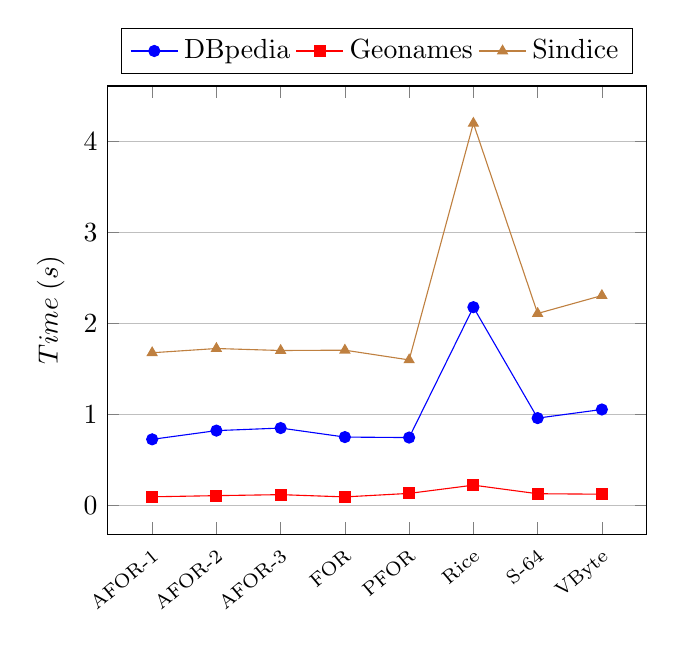
\begin{tikzpicture}
\begin{axis}[
ylabel=$Time \; (s)$,
x tick label style={font=\scriptsize, rotate=40, anchor=north east},
xtick={1,...,8},
xticklabels={AFOR-1, AFOR-2, AFOR-3, FOR, PFOR, Rice, S-64, VByte},
legend style={at={(0.5,1.13)}, anchor=north, legend columns=-1},
%ybar,
ymajorgrids=true,
%bar width=5pt,
]

\addplot[blue,mark=*]
coordinates {(1, 0.7267) (2, 0.8225) (3, 0.8506) (4, 0.7516) (5, 0.7462) (6, 2.1778) (7, 0.9598) (8, 1.0544) };
\addplot[red,mark=square*]
coordinates {(1, 0.0959) (2, 0.1085) (3, 0.1196) (4, 0.0947) (5, 0.1333) (6, 0.2237) (7, 0.1296) (8, 0.1245)};
\addplot[brown,mark=triangle*]
coordinates {(1, 1.6773) (2, 1.7239) (3, 1.702) (4, 1.7056) (5, 1.5986) (6, 4.1963) (7, 2.1086) (8, 2.3053)};

\legend{DBpedia, Geonames, Sindice}

\end{axis}
\end{tikzpicture}%
